\section{Teori}

\subsection{Euler-Bernoulli}
Flere av oppgavene i denne rapporten omhandler Euler-Bernoulli-bjelken. I følge Wikipedia er dette en grunnleggende metode for å regne ut hvor mye en bjelke av et gitt materiale bøyer seg under press. Metoden er oppkalt etter Jacob Bernoulli som gjorde de største oppdagelsene, det var derimot ikke før rundt 1750 at Leonhard Euler og Daniel Bernoulli kom opp med en komplett teori. Metoden ble ikke brukt i praksis på noen større prosjekter før byggingen av Eiffeltårnet i 1889, men har siden blitt en hjørnestein innen ingeniørkunsten.\footnote{\url{https://en.wikipedia.org/wiki/Euler-Bernoulli_beam_theory}, (14.04.2016)} Euler-Bernoulli-likningen er som følger:
\begin{quote}
\begin{equation}
EIy''''=f(x)
\end{equation}
\end{quote}
Den vertikale forskyvningen av en $L$ meter lang bjelke, oppfyller likningen når $0\leq x\leq L$. Likningen inneholder noen konstanter; $E$ er en materialkonstant kalt Youngmodulusen. $I$ er et arealmoment til bjelkens tverrsnitt normalt på lengderetningen. $I$ er konstant langs hele bjelken. Høyresiden av likningen, $f(x)$, er en kraft som virker på bjelken per lengde-enhet målt i Newton per meter. Kraften inkluderer vekten til bjelken. Dette har vi fra læreboken.\footnote{Sauer, Timothy, (2012) Numerical Analysis second edition, side 102-.}

Hvorfor kan dette brukes på stupebrett?
Legge til ekstra kraft for haug og person.

\subsection{Taylors Teorem}
Taylors Teorem er en måte å estimere en gitt funksjon på ved hjelp av polynomer. Man kan se på Taylors formel som en generalisering av "Mean Value Theorem", som sier at dersom funksjonen f er kontinuerlig i et lukket intervall [a,b] og f er deriverbar i det åpne intervallet (a,b), et punkt c, a < c < b eksisterer slik at :
\begin{quote}
\begin{equation}
f'(c) = \frac{f(b) - f(a)}{b-a}
\end{equation}
\end{quote}
Mer bestemt, la f være en funksjon slik at f og dens første n-deriverte er kontinuerlig i [a,b]. Videre, la $f^{(n+1)}(x)$ eksistere for alle x i (a,b). Da eksisterer det et tall c i (a,b) slik at:
\begin{quote}
\begin{equation}
f(b) = f(a) + (b-a) \frac{f'(a)}{1!} + (b-a)^2 \frac{f''(a)}{2!} + .... + (b-a)^n \frac{f^{(n)}}{n!} + (b-a)^{(n+1)} \frac{f^{(n+1} (c)}{(n+1)!}
\end{equation}
\end{quote}
Formelen sier også at dersom b < a, så vil [a,b] og (a,b) blir byttet ut med [b,a] og (b,a) henholdsvis. Man kan også se at dersom vi bytter ut b med x, står vi igjen med Taylor's formelen. \\
En annen måte å skrive Taylor's formelen på er
\begin{quote}
\begin{equation}
\sum_{i=0}^n (x-a)î \frac{f''(a)}{i!} + (x-a)^{n+1} \frac{f^{(n+1)} (c) }{(n+1)!}
\end{equation}
\end{quote}
som også er kjent som n-te grad Taylor polynom (eller Taylor serie) med feil ledd.\\
For å visualisere dette kan vi ta for oss funksjonen $f(x) = sin(x)$. Ved å regne ut flere ledd i Taylor-rekken vil vi kunne skape en tilnærming av funksjonen. Desto flere ledd, desto mer nøyaktig tilnærming:

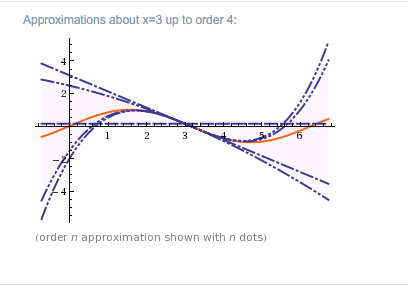
\includegraphics[width=\textwidth]{taylor_sinx}
Grafen er en taylors-rekke av f(x) = sin(x), der x=3. Studerer man de blå striplette linjene ser vi at de inneholder ulikt antall prikker. 1 prikk tilsvarer første deriverte, 2prikker tilsvarer andre deriverte osv. Ut i fra grafen ser man at dersom man har et høyere derivasjonsledd vil den blå linjen følge funksjonen mer og mer, og vi får en mer nøyaktig tilnærming av funksjonen. 
 
 \subsection{Kondisjonstall}
 Når vi snakker om kondisjonstallet til en funksjon f med et argument x måler vi omfanget av endringer til f med liten endring i x. Vi bruker dette til å se hvor sensitiv en funksjon er til endringer eller feil i x og størrelsen på feil som kan forekomme i f. Man skulle tro at en liten endring i x ikke vil ha et stort utfall på effekten til f, men dette skal vi vise kan bli ganske storslåtte. I matrisesammenheng kan vi se på den lineære likningen Ax = b. Kondisjonstallet til A vil fortelle oss om hvor store endringene i b blir med små endringer i x. I MATLAB benytter vi oss av Cond(A) for å finne kondisjonstallet. Denne metoden bygger på funksjonen:
 \
 \begin{equation}
 Cond(A) = ||A^{-1}|| \cdot ||A||
 \end{equation}

\subsection{Feil}
Forover og bakoverfeil.

\subsection{MATLAB}

\subsection{Teori tilknyttet oppgaver}
\subsubsection{Oppgave 3}
Møtte på et problem tilknyttet oppgave 3 hvor vi fikk positive verdier for y. Etter lang leting viste det seg at i vår lagA- metode så hadde vi klart å skreve -157/17 kontra -156/17 som det egentlig skulle være. Var spennende å se at en så liten feil kunne resultere til så forskjellige verdier. 

For å løse de vanskeligste problemene i dette prosjektet, trenger vi hjelp fra et digitalt verktøy. Og vi bruker MatLab. MatLab, kort for Matrix Laboratory, er et omfattende matematikk-program utiklet av MathWorks. Siden programmet først ble utgitt i 1984 har det blitt et veldig populært program til bruk på utdanningsinstitusjoner. I 2004 hadde MatLab over 1 million registrerte lisenser på verdensbasis.
MatLab opererer med et eget script-språk basert på programmeringsspråket C, så det er veldig nyttig for oss dataingeniører. Med MatLab kan vi utføre matriseregning, behandle og plotte funksjoner, implementere algoritmer osv. Det at det opererer på et script-språk gjør også at vi kan skrive egne funksjoner for å løse problemer. Ved å skrive kode for å løse oppgavene er det lett for oss å vise fremgangsmåte i tillegg til riktig svar.

\subsubsection{Oppgave 5}
Vi starter her med å hente inn konstantene vi fikk oppgitt i boken, deretter har vi definert at $n=10*2^{i}$ som oppgitt i oppgaven og bruker ebbeam-funksjon som er 
Euler-Bernoulli sin metode for å beregne hvor mye materialet bøyer seg under press. 
Vi beregner den numeriske løsningen ved hjelp ebbeam-funksjonen, den faktiske løsningen, feilen og kondisjonstallet. 
\begin{lstlisting}
format long;
[E, I, D, d, w, f, g, L, p] = hentKonstanter();
n = 10;

i_max = 11;

n = zeros(i_max, 1);
y_num_L = zeros(i_max, 1);
y_actual_L = zeros(i_max, 1);
error = zeros(i_max,1);
cond_A = zeros(i_max,1);

syms y(x) y(z);
y(x) = correct_y(f,E,I,L,x);

for i = (1:i_max)
    n(i) = 10*2^i;
    y_num = ebbeam(L,n(i),f,E,I);
    y_num_L(i) = y_num(n(i));
    y_actual_L(i) = y(L);
    error(i) = abs(y_actual_L(i) - y_num(n(i)));
    A = lagA(n(i));
    cond_A(i) = condest(A);
end

T = table(n, y_num_L, y_actual_L, error, cond_A);
disp(T);
figure;
plot(log(n), log(error));
hold on;
plot(log(n), log(cond_A));
title('Error figure and Condition Number - Oppgave 5');
\end{lstlisting}

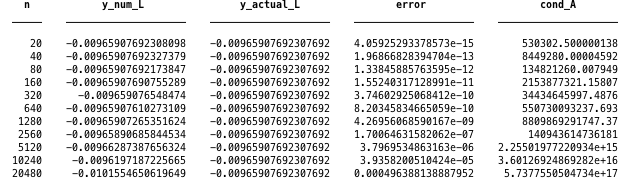
\includegraphics[width=\textwidth]{Oppgave5}
Ut i fra resultatet over er det lett å se hvilken n-verdi som gir størst feil, når n = 20. Man ser også at når n øker så minker feilen, dette er fordi jo flere intervaller vi har jo mer nøyaktig blir estimeringen. Kondisjonstallet til A ser vi også ut i fra resultatet at den stiger kontinuerlig når n øker. \\
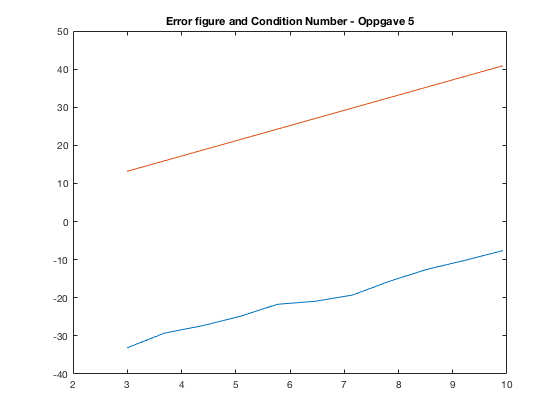
\includegraphics[width=\textwidth]{Oppgave5fig}
Grafen viser kondisjonstallet i en rett linje (rød), mens den blå linjen er feilen. Vi ser at når n øker minsker feilen og beveger seg mot 0, mens kondisjonstallet forsetter å øke kontinuerlig. 